\pagebreak
\section{Deadlocks} \label{deadlocks}
In questo capitolo cercheremo di approfondire i deadlocks: capiremo sotto quali condizioni si giungerà ad una soluzione di deadlock e i diversi algoritmi per la gestione dei deadlocks.

\subsubsection*{Modello di sistema}
Prima di discutere effettivamente dei deadlock è importante fare un piccola premessa. In questo capitolo avremo a che fare con sistemi che possono essere composti da \textit{m} tipi di risorse generiche: queste potrebbero essere dei dispositivi I/O, dati su disco, delle allocazioni in memoria, la CPU oppre dei semafori generici. Queste risorse vengono definite con la notazione $R_m$. Inoltre, ogni tipo di risorsa può essere \textbf{singolo}, come un slot del DVD sul computer, oppure \textbf{multiplo} come la presenza di diverse porte USB oppure molti buffer in memoria.
% 
\subsection{Nozioni fondamentali}
Ripassiamo innanzitutto il concetto di deadlock. Prendiamo il caso in cui due semafori $S_1$ ed $S_2$, entrambi inizializzati a 1, siano condivisi da due thread $T_1$ e $T_2$. Osservando lo pseudo-codice seguente, si ha una classica situazione di deadlock. Se $T_1$ e $T_2$ sono eseguiti contemporaneamente, $T_1$ occupa subito $S_1$ e $T_2$ occupa subito $S_2$. Dopo di che $T_1$ aspetta $S_2$ che però è occupato da $T_1$ il quale è in attesa di $S_1$, occupato da $T_1$. Siamo quindi in una situazione di stallo dove entrambi i thread stanno aspettando l'altro e nessuno dei due termina l'esecuzione

\begin{lstlisting}[caption = {Classica situazione di deadlock}]
/* T1 */
    wait(S1); /* occupa S1 */
    wait(S2); /* aspetta per S2 */

/* T2 */
    wait(S2); /* occupa S2 */
    wait(S1); /* attende S1 */
\end{lstlisting}
% 

% 
\subsubsection{Caratterizzazione}\label{4_punti_deadlock}
Possiamo osservare che si devono verificare 4 condizioni affinché si arrivi ad una situazione di deadlock.
\vspace{-5px}
\begin{enumerate}
    \setlength{\itemsep}{-.15 em}
    \item \textbf{Mutua esclusione}: banalmente, ci deve essere almeno una risorsa che sia utilizzata da un thread alla volta;
    \item \textbf{Hold and wait}: deve esistere almeno un thread che sta cercando di accedere alla risorsa che è già occupata e, di conseguenza, deve attendere;
    \item \textbf{No preemption}: una risorsa può essere rilasciata volontariamente dei thread. Le risorse non possono quindi essere "rubate" da altri thread e, di conseguenza, un thread non può essere spezzato durante la sua fase critica;
    \item \textbf{Attesa circolare}: è il requisito più importante, deve verificarsi una situazione come quella dei cinque filosofi (paragrafo \ref{5_filosofi}), ovvero che un thread attende la conclusione di un altro thread che ... che aspetta la conclusione del thread iniziale.
\end{enumerate}
Se almeno una di queste quattro condizioni \textbf{non} è \textbf{verificata} allora non si è in una situazione di deadlock.

% 
\subsubsection{Grafo risorsa-allocazione}
Uno strumento molto importante, utile per visionare i diversi casi di deadlock è il grafo risorsa-allocazione. Questo grafo è composto, come ogni grafo, da vertici e archi. I vertici si suddividono in due tipi: il primo tipo rappresenta la risorsa $R_m$ mentre il secondo tipo indica il thread $T_n$. Il grafo è \textbf{diretto}, ciò significa che gli archi hanno una direzione. In particolare $R \to T$ indica che il thread $T$ detiene/occupa la risorsa $R$, mentre $T \to R$ segnala che il thread $T$ è in attesa della risorsa $R$. Inoltre, si osserva che generalmente i vertici che rappresentano una risorsa multipla contengono tanti pallini ($\bullet$) quante sono le istanze di quella risorsa disponibili (come le 5 porte USB). 

Prendiamo come esempio la figura \ref{fig:grafo_deadlock}. Possiamo notare che rispetta tutte "regole" del grafo risorsa-allocazione. In particolare possiamo affermare che $R_1$ ed $R_3$ sono risorse singole mentre $R_2$ ed $R_4$ sono risorse multiple (con, rispettivamente, 2 e 4 istanze).
\begin{figure}[h]
    \centering
    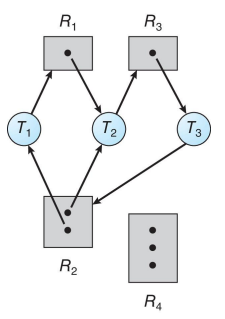
\includegraphics[width = .35 \textwidth]{../res/imgs/deadlocks/deadlock_graph.png}
    \caption{Rappresentazione grafica di un grafo che presenta una situazione di deadlock.}
    \label{fig:grafo_deadlock}
\end{figure}
Inoltre possiamo dire che ci troviamo in una situazione di \textit{deadlock}. Perché? Partiamo da $R_2$, questa è occupata da $T_1$ e $T_2$; $T_1$ è in attesa di $R_1$ la quale è occupate da $R_2$ che, a sua volta, sta aspettando che $R_3$ venga liberata da $T_3$ il quale sta attendendo la liberazione due $R_2$, occupata per l'appunto da $T_1$ e $T_2$. È proprio una situazione di deadlock: a primo impatto possiamo dire ciò perché è presente un \textbf{ciclo}. Osservando però la figura \ref{fig:grafo_no_deadlock}, capiamo che il fatto che ci sia un ciclo non implica che ci sia per forza una situazione di deadlock.
\begin{figure}[h]
    \centering
    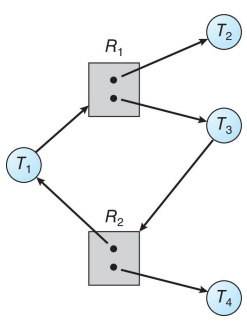
\includegraphics[width = .35\textwidth]{../res/imgs/deadlocks/no_deadlock_graph.png}
    \caption{Rappresentazione grafica di un grafo senza deadlock.}
    \label{fig:grafo_no_deadlock}
\end{figure}
Se osserviamo infatti la figura \ref{fig:grafo_no_deadlock} riconosciamo che prima o poi il thread $T_2$ oppure $T_4$ rilascerà la risorsa e di conseguenza le richiesta degli altri thread saranno soddisfatte.

Riassumiamo ora queste informazioni nel seguente diagramma: 
\begin{figure}[h]
    \centering

    \begin{tikzpicture}
  [
    grow                    = down,
    sibling distance        = 10em,
    level distance          = 6em,
    edge from parent/.style = {draw, -latex},
    every node/.style       = {font=\footnotesize},
    sloped
  ]
  \node [root] {Contiene cicli?}
    child { node [env] {Non ci sono\\deadlock.}
      edge from parent node [above] {No} }
    child { node [env] {Ci sono\\solo risorse\\singole?}
      child { node [env] {È possibile\\che ci siano,\\non è sicuro.} edge from parent node [above] {No}}
      child {node [env] {Ci sono\\sicuramente\\deadlock.} edge from parent node [above] {Si}}
              edge from parent node [above] {Si}};
\end{tikzpicture}
    
    \caption{Piccolo \textit{decision tree} utile per capire se è presente un deadlock oppure no.}
    \label{fig:deadlock_decision_tree}
\end{figure}
% 
\subsubsection*{Livelock}
Oltre al deadlock esiste anche una seconda situazione di stallo chiamata \textit{livelock}. In questo caso i due processi non sono completamente in una situazione di stallo ma non riescono a terminare la loro esecuzione. Possiamo allegoricamente spiegare queste situazione con un corridoio dove ci sono due persone, A e B, che vanno in direzione opposta. Ad un certo punto, nel tempo, si incontrano, allora, per non scontrarsi, A si sposta, ma contemporaneamente lo fa anche B. A questo punto A si sposta di nuovo, ma lo fa anche B. I due processi quindi si ostacolano l'un l'altro non riuscendo a terminare. 
% 
\subsection*{Prevention}
Come vedremo in questo capitolo, ci sono diversi metodi finalizzati alla gestione dei deadlock. Il primo metodo che andiamo a discutere è quello di "prevenzione". In essenza, questo metodo si occupa di \textbf{invalidare} una delle quattro \textbf{condizioni} necessarie che generano una situazione di deadlock (vedi paragrafo \ref{4_punti_deadlock}). Anticipiamo già che questo approccio non è assolutamente efficiente e non è utilizzato.

\begin{enumerate}
    \item La prima condizione, ovvero quella di mutua esclusione raramente può essere invalidata. Proprio perché la sincronizzazione tra processi nasce proprio per far si che solo un processo abbia accesso ad una risorsa, la mutua esclusione è fondamentale. Altrimenti si incombe in situazioni dove più processi sono, per esempio, in scrittura, sullo stesso file.
    
    \item Per quanto riguarda l'\textit{hold and wait}, in questo caso si cerca di fare in modo che un processo che detiene una risorsa non ne può richiedere un'altra (si rimuove l'\textit{hold} dalla definizione). Di conseguenza si fa in modo che un thread, prima di essere eseguito, faccia una richiesta contemporanea a tutte le risorse di cui ha bisogno lasciano tutti gli altri processi ad aspettare. Si entra in una situazioni di inefficienza e, talvolta, c'è il rischio che un processo vada in \textbf{starvation}.

    \item Affine di invalidare il punto tre si aggiunge la \textit{preemption}, ovvero che i processi possono essere interrotti al fine di lasciare la risorsa ad altri processi. Anche in questo caso però si possono verificare situazioni assurde: si pensi all'utilizzo di una stampante, un thread non può fermare la stampa e iniziare a stampare. Si ha anche in questo caso una soluzione poco ottimale.

    \item Solo nel quarto punto, dove si cerca di evitare l'attesa circolare si ha effettivamente una soluzione sensata. Nella pratica si cerca di eliminare la circolarità imponendo dei vincoli particolare ai processi, per esempio un \textbf{ordine} di esecuzione. 
\end{enumerate}

% 
\subsection{Avoidance}\label{avoidance}
Il secondo approccio che andremo a discutere più a fondo è una sorta di miglioramento della prevenzione. In questo caso si cerca proprio di \textbf{evitare} di ricadere in situazioni che possono portare al deadlock, è una prevenzione molto più \textit{strict}.

Affinché questo approccio funzioni però deve essere fornita un'informazione importante da parte del processo, ovvero il numero massimo di risorse per tipo che il processo necessita durante la sua esecuzione. Per esempio, 6 risorse di tipo A, 5 risorse di tipo B e 2 risorse di tipo C.

\subsubsection{Safe state}
Il safe state, ovvero lo \textbf{stato sicuro}, è una situazione in cui esiste un ordine di esecuzione di thread secondo il quale tutti i thread possono essere completati uno dopo l'altro. Quando un processo fa la richiesta per le risorse, prima di concederle, l'algoritmo (che vedremo in seguito ) controlla se dopo la cessione delle risorse si è in una situazione ancora safe. Se si, allora le risorse vengono occupate dal processo, altrimenti il processo deve aspettare il termine di alcuni thread.

Nella primo grafo della figura \ref{fig:safe_unsafe} si è in una condizione non sicura in quanto non esiste una sequenza di esecuzione dei processi dove non si verifichi una situazione di deadlock. 
\begin{figure}[h]
    \centering
    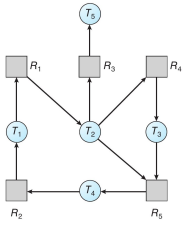
\includegraphics[width = .35\textwidth]{../res/imgs/deadlocks/unsafe.png}
    \hspace{5em}
    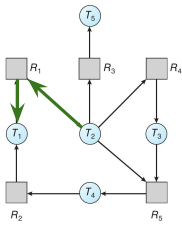
\includegraphics[width = .35\textwidth]{../res/imgs/deadlocks/safe.png}
    \caption{Differenza tra situazione unsafe e safe.}
    \label{fig:safe_unsafe}
\end{figure}
Nel secondo grafo invece si è in una situazione safe in quanto esiste una sequenza dove tutti i processi possono essere eseguiti senza entrare in una condizione di deadlock: $T_1 \to T_4 \to T_3 \to T_5 \to T_2$ infatti è una sequenza che permette il completamento dell'esecuzione dei threads. Anche in questo caso possiamo riassumere tutto in un piccolo \textit{decision tree}:
\begin{figure}[h]
    \centering

    \begin{tikzpicture}
  [
    grow                    = down,
    sibling distance        = 10em,
    level distance          = 6em,
    edge from parent/.style = {draw, -latex},
    every node/.style       = {font=\footnotesize},
    sloped
  ]
  \node [root] {Sei in un safe state?}
    child { node [env] {È possibile\\che ci siano,\\non è sicuro.}
        edge from parent node [above] {No}}
    child { node [env] {Non ci sono\\deadlock.}
      edge from parent node [above] {Si} };
\end{tikzpicture}
\end{figure}

\noindent Ricordiamo infine che gli algoritmi che vedremo in questo paragrafo al fine di prevenire i deadlock \textbf{evitano} di entrare in \textbf{unsafe state}, rimanendo quindi in safe state.
% 
\subsubsection{Algoritmo sul grafo risorsa-allocazione}
Iniziamo con un algoritmo che funziona solo nel caso di \textbf{risorse singole}, ovvero nel caso in cui si ha solo un pallino ($\bullet$) nel grafo, e quindi ogni tipi di risorsa ha una sola istanza. Introduciamo ora la nozione di \textbf{claim edge} ovvero un arco tratteggiato che indica che il processo $T_i$ può richiedere la risorsa $R_j$. Questi archi diventano \textbf{request edge} nel momento in cui si effettua la richiesta e poi si trasformano a loro volta in \textbf{assignements edge} nel momento in cui stanno utilizzando la risorsa. Osservando il grafo in figura \ref{fig:claim_edge} notiamo che $T_1 \to R_2$ è un claim edge, $T_2 \to R_1$ è un request edge e $R_1 \to T_1$ è un assigmenent edge. 
\begin{figure}[h]
    \centering
    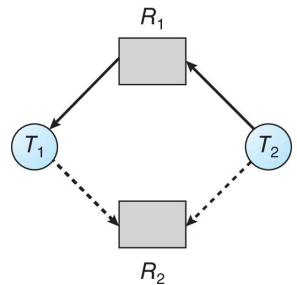
\includegraphics[width = .4\textwidth]{../res/imgs/deadlocks/claim_edge.png}
    \caption{Un grafo composto da tutti e tre i tipi di archi.}
    \label{fig:claim_edge}
\end{figure}

Nella situazione presentata in figura \ref{fig:claim_edge}, si rischia di essere in una situazione \textit{unsafe}. Questo perché se $R_2$ è assegnata al thread $T_2$ nel caso in cui il thread $T_1$ effettui la richiesta per $R_2$ si è in una situazione di deadlock. Possiamo infatti osservare che si ha la presenza di un ciclo e che tutte le risorse abbiano un'istanza, facendo riferimento allo schema in figura \ref{fig:deadlock_decision_tree}, si ha che si è sicuramente in una situazione di deadlock. Ponendo infatti che $R_2$ venga assegnata a $T_2$, nel momento in cui $T_1$ effettui una richiesta, l'algoritmo la nega, in modo tale da non essere in una situazione di deadlock.
\begin{figure}[h]
    \centering
    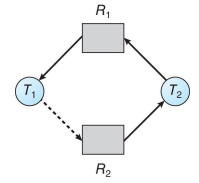
\includegraphics[width = .4\textwidth]{../res/imgs/deadlocks/request_denied.png}
    \caption{L'algoritmo nega la richiesta di $T_1$ per $R_2$}
    \label{fig:request_denied}
\end{figure}
% 
\subsubsection{Algoritmo del banchiere}
Passiamo ora ad una situazione più reale, quella in cui esistono più risorse con più istanze ciascuna. L'algoritmo a cui si fa affidamento è detto \textit{Banker's algorithm}, ovvero l'algoritmo del banchiere.

Innanzitutto, definiamo con $n$ il numero di processi ed $m$ il numero di tipi di risorse; definiamo poi tre matrici e un'array, strutture sul quale l'algoritmo si appoggia:
\vspace{-15pt}
\begin{itemize}
\setlength{\itemsep}{-.15 em}
    \item L'array \textbf{avaiable} (disponibili) che indica quante istanze di risorse sono disponibili per ogni tipo. Per esempio, la risorsa $j$ ha a disposizione 3 istanze, e questo $\forall j\in[0,m]$.
    \item La prima matrice, \textbf{max} che indica il massimo numero di istanze della risorsa $j$esima che il processo $i$esimo ha al più bisogno ($\forall i\in[0,n]$).
    \item La seconda matrice \textbf{allocated} (allocato), che indica quante istanze della risorsa $j$esima il processo $i$esimo ha già allocato.
    \item La terza matrice, \textbf{need} (bisogno), che non è altro che la differenza tra $max$ e $allocated$; questa matrice indica di quante altre istanze della risorsa $j$esima il processo $i$esimo potrebbe, al più, aver bisogno.
\end{itemize}

Per capire l'algoritmo al meglio si può tranquillamente trascurare lo pseudo-codice e partire subito con un \textbf{esempio}. Abbiamo $n = 5$ thread, da $T_0$ a $T_4$, e 3 tipi di risorse: A, con 10 istanze, B, con 5 e C, che ha a disposizione 7 istanze. Al tempo iniziale $t_0$, la situazione è la seguente:
\begin{table}[!h]
    \centering
    \begin{tabular}{c}
         \underline{\textit{Threads}} \\\\ $T_0$ \\ $T_1$ \\ $T_2$ \\ $T_3$ \\ $T_4$
    \end{tabular}
    \begin{tabular}{c c c}
         \multicolumn{3}{c}{\underline{\textit{Allocated}}} \\
         \textbf{A} & \textbf{B} & \textbf{C} \\
         0 & 1 & 0 \\
         2 & 0 & 0 \\
         3 & 0 & 2 \\
         2 & 1 & 1 \\
         0 & 0 & 1
    \end{tabular}
    \hspace{5px}
    \begin{tabular}{c c c}
         \multicolumn{3}{c}{\underline{\textit{Max}}} \\
         \textbf{A} & \textbf{B} & \textbf{C} \\
         7 & 5 & 3 \\
         3 & 2 & 2 \\
         9 & 0 & 2 \\
         2 & 2 & 2 \\
         4 & 3 & 3 \\
    \end{tabular}    
\end{table}

\noindent Un esempio di lettura della tabella è il seguente: $T_0$ detiene un'istanza di tipo B e zero istanze di tipo A e C. Può richiedere un massimo di 7 istanze di tipo A, 5 istanze di tipo B e 3 istanze di tipo C.

Con questi dati possiamo ora calcolare le due strutture che ci mancano: \textit{Avaiable} e \textit{Need}, che rispettivamente indicano le risorse che sono disponibili (per ogni tipo) e il numero di risorse che un determinato thread può richiedere. Osserviamo che per calcolare il vettore di risorse disponibili è necessario sottrarre alle istanze iniziali la somma delle risorse occupate dai threads. Per esempio, nel caso delle istanze disponibili della risorsa A abbiamo che sono $10 - (2 + 3 + 2) = 3$, occupate rispettivamente da: $T_1$, $T_2$ e $T_3$. per calcolare invece la matrice \textit{Need}, per ogni cella della matrice si sottrarre il valore di \textit{Max} al valore di $Allocated$ nella cella $[i,j]$.
\begin{table}[h!]
    \centering
        \begin{tabular}{c c c}
         \multicolumn{3}{c}{\underline{\textit{Avaiable}}} \\
         \textbf{A} & \textbf{B} & \textbf{C} \\
         3 & 3 & 2
    \end{tabular}
    \hspace{5pt}    
    \begin{tabular}{c c c}
         \multicolumn{3}{c}{\underline{\textit{Need}}} \\
         \textbf{A} & \textbf{B} & \textbf{C} \\
         7 & 4 & 3 \\
         1 & 2 & 2 \\
         6 & 0 & 0 \\
         0 & 1 & 1 \\
         4 & 3 & 1 \\
    \end{tabular}
\end{table}

Abbiamo ora tutte le risorse necessarie per iniziare a eseguire l'algoritmo. Iniziamo scorrendo la matrice \textit{Need} e comparandola con il vettore \textit{Avaiable}. Partiamo dal thread $T_0$: con le risorse disponibili $[3,3,2]$, il thread ha la possibilità di terminare? No, perché per terminare necessita, al più, di 7 istanze di A, 4 istanze di B e 3 istanze di C. Passiamo ora al secondo thread: $T_1$ può terminare con le risorse disponibili? Si, perché tutte le risorse di cui ha bisogno sono $\leq$ rispetto alle risorse disponibili. A questo punto allora si spostano le risorse necessarie a $T_1$ per terminare, ovvero $[1,2,2]$:

\begin{table}[h]
    \centering
    \begin{tabular}{c}
         \underline{\textit{Threads}} \\\\ $T_0$ \\ $T_1$ \\ $T_2$ \\ $T_3$ \\ $T_4$
    \end{tabular}
    \begin{tabular}{c c c}
         \multicolumn{3}{c}{\underline{\textit{Allocated}}} \\
         \textbf{A} & \textbf{B} & \textbf{C} \\
         0 & 1 & 0 \\
         \textbf{3} & \textbf{2} & \textbf{2} \\
         3 & 0 & 2 \\
         2 & 1 & 1 \\
         0 & 0 & 1
    \end{tabular}
    \hspace{5px}
    \begin{tabular}{c c c}
         \multicolumn{3}{c}{\underline{\textit{Max}}} \\
         \textbf{A} & \textbf{B} & \textbf{C} \\
         7 & 5 & 3 \\
         3 & 2 & 2 \\
         9 & 0 & 2 \\
         2 & 2 & 2 \\
         4 & 3 & 3 \\
    \end{tabular}    
    \hspace{5pt}    
    \begin{tabular}{c c c}
         \multicolumn{3}{c}{\underline{\textit{Need}}} \\
         \textbf{A} & \textbf{B} & \textbf{C} \\
         7 & 4 & 3 \\
         0 & 0 & 0 \\
         6 & 0 & 0 \\
         0 & 1 & 1 \\
         4 & 3 & 1 \\
    \end{tabular}
    \hspace{5pt}
    \begin{tabular}{c c c}
         \multicolumn{3}{c}{\underline{\textit{Avaiable}}} \\
         \textbf{A} & \textbf{B} & \textbf{C} \\
         \textbf{2} & \textbf{1} & \textbf{0}
    \end{tabular}
\end{table}
\pagebreak Una volta terminato il thread $T_1$, le risorse vengono rilasciate e il vettore \textit{Avaiable} va aggiornato, sommando alle risorse disponibili le risorse che sono appena state rilasciate da $T_1$.
\begin{table}[h!]
    \centering
    \begin{tabular}{c c c}
         \multicolumn{3}{c}{\underline{\textit{Avaiable}}} \\
         \textbf{A} & \textbf{B} & \textbf{C} \\
         5 & 3 & 2
    \end{tabular}
\end{table}

A questo punto ci sono abbastanza risorse per terminare un altro processo come, per esempio $T_3$ oppure $T_4$. Così facendo, mano che i thread vengono eseguiti e terminati vengono rilasciate abbastanza risorse per completare quelli più onerosi. Una sequenza esempio dell'ordine con il quale i thread sono completati può essere: \{$T_1,T_3,T_4,T_2,T_0$\}. 

Può succedere che durante l'esecuzione dei thread possono arrivare altre richieste che devono essere accettate o meno. Per esempio se prima dell'esecuzione $T_4$ avesse fatto una richiesta $[3,3,0]$, la richiesta sarebbe stata rifiutata dato che le risorse disponibili erano minori rispetto alla richiesta.
% 
\subsection{Detection}
L'ultimo approccio che andiamo a discutere è il rilevamento del deadlock: si va alla ricerca di tale e, una volta trovato, si passa al salvataggio, alla \textbf{recovery}. Anche in questo caso, come per l'approccio di \textit{avoidance} (paragrafo \ref{avoidance}) sono presenti due algoritmi, uno studiato per avere solo un'istanza per risorsa e il secondo che copre anche il caso in cui ci siano più istanze per risorse.



\subsubsection{Istanza singola}
In questo primo caso si fa riferimento ad un secondo grafo particolare chiamato \textbf{wait-for graph}. È una modifica del \textit{resource-allocation graph} dove si evidenzia il fatto che un thread sta aspettando il termine dell'esecuzione di un altro thread: non sono infatti presenti vertici che rappresentano risorse a ci sono solo nodi che indicano i thread.
\begin{figure}[h]
    \centering
    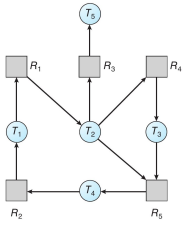
\includegraphics[width = .25\textwidth]{../res/imgs/deadlocks/unsafe.png}
    \hspace{10pt}
    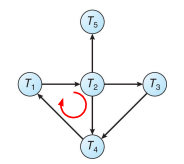
\includegraphics[width = .35\textwidth]{../res/imgs/deadlocks/wait-for_graph.png}
    \caption{Un grafo \textit{resource-allocation} e il suo rispettivo \textit{wait-for graph}}
    \label{fig:wait-for}
\end{figure}
In figura \ref{fig:wait-for} si osserva la traduzione di un grafo risorsa allocazioni in gra grafo \textit{wait-for}. Si nota che nel secondo grafo si accetua ancora di più la presenza di cicli e, dato che is tratta di risorse con istanza singola, la presenza di un ciclio ha l'immediata conseguenza di generare una situazione di deadlock.

L'algoritmo di cui stiamo parlando infatti, per rilevare un deadlock, si limita a creare un \textit{wait-for graph} e controllare la presenza di cicli\footnote{Da studente che ha seguito il corso "Dati e Algoritmi" penso che si utilizzino algoritmi basati su BFS oppure DFS.}. Una volta trovato il ciclo si è sicuri di aver trovato il deadlock e si passa alla \textit{deadlock recovery} (vedi paragrafo \ref{recovery}). Possiamo quindi notare che nella figura \ref{fig:wait-for} si è in una condizione di deadlock dato che il thread $T_1$ sta attendendo il termine di $T_2$ che è in attesa di $T_4$ che a sua volta sta aspettando $T_1$. Una situazione analoga è presente anche con i thread $T_1,T_2,T_3,T_4$.
% 
\subsubsection{Istanze multiple}
Nel caso invece delle istanze multiple, anche in questo algoritmo si fa affidamento a diverse strutture dati, proprio come nell'algoritmo del banchiere. Avremo quindi a che vedere con $n$ processi che hanno a che fare con $m$ tipi di risorse che interagiranno con due matrici e un vettore.
\vspace{-5px}
\begin{itemize}
\setlength{\itemsep}{-.15 em}
    \item Il vettore \textit{Avaiable}, proprio come nell'algoritmo del banchiere, tiene traccia di quante istanze sono libere per ogni tipo di risorsa.
    \item La prima matrice \textit{Allocated} memorizza il numero di risorse che ogni processo detiene.
    \item La seconda matrice, \textbf{Request}, indica quante risorse il thread sta richiedendo al fine di terminare.
\end{itemize}

Come nel caso dell'algoritmo del banchiere, non ci soffermiamo sullo pseudo-codice ma partiamo subito con un esempio. Poniamo di avere cinque threads, da $T_0$ a $T_4$ e di avere anche in questo caso tre tipi di risorse: A, con 7 istanze, B con 2 istanze e C con 6 istanze. Al tempo iniziale $t_0$ ci troviamo nella seguente situazione:
\begin{table}[h]
    \centering
    \begin{tabular}{c}
         \underline{\textit{Threads}} \\\\ $T_0$ \\ $T_1$ \\ $T_2$ \\ $T_3$ \\ $T_4$
    \end{tabular}
    \begin{tabular}{c c c}
         \multicolumn{3}{c}{\underline{\textit{Allocated}}} \\
         \textbf{A} & \textbf{B} & \textbf{C} \\
         0 & 1 & 0 \\
         2 & 0 & 0 \\
         3 & 0 & 3 \\
         2 & 1 & 1 \\
         0 & 0 & 2 \\
    \end{tabular}
    \hspace{5px}
    \begin{tabular}{c c c}
         \multicolumn{3}{c}{\underline{\textit{Request}}} \\
         \textbf{A} & \textbf{B} & \textbf{C} \\
         0 & 0 & 0 \\
         2 & 0 & 2 \\
         0 & 0 & 0 \\
         1 & 0 & 0 \\
         0 & 0 & 2 \\
    \end{tabular} 
    \hspace{5pt}
    \begin{tabular}{c c c}
         \multicolumn{3}{c}{\underline{\textit{Avaiable}}} \\
         \textbf{A} & \textbf{B} & \textbf{C} \\
         0 & 0 & 0 
    \end{tabular}
\end{table}

\noindent Dalla tabella \textit{Request} possiamo notare che sia $T_0$ che $T_2$ possono completare senza attendere altri processi dato che non richiedono nulla. Una volta terminati $T_0$ e $T_2$ tutti gli altri thread possono man mano terminare. Non siamo quindi in una situazione di deadlock.

Mettiamoci però nel caso in cui $T_2$ debba richiedere una risorsa di tipo C.
\begin{table}[h]
    \centering
    \begin{tabular}{c}
         \underline{\textit{Threads}} \\\\ $T_0$ \\ $T_1$ \\ $T_2$ \\ $T_3$ \\ $T_4$
    \end{tabular}
    \begin{tabular}{c c c}
         \multicolumn{3}{c}{\underline{\textit{Allocated}}} \\
         \textbf{A} & \textbf{B} & \textbf{C} \\
         0 & 1 & 0 \\
         2 & 0 & 0 \\
         3 & 0 & 3 \\
         2 & 1 & 1 \\
         0 & 0 & 2 \\
    \end{tabular}
    \hspace{5px}
    \begin{tabular}{c c c}
         \multicolumn{3}{c}{\underline{\textit{Request}}} \\
         \textbf{A} & \textbf{B} & \textbf{C} \\
         0 & 0 & 0 \\
         2 & 0 & 2 \\
         0 & 0 & \textbf{1} \\
         1 & 0 & 0 \\
         0 & 0 & 2 \\
    \end{tabular} 
    \hspace{5pt}
    \begin{tabular}{c c c}
         \multicolumn{3}{c}{\underline{\textit{Avaiable}}} \\
         \textbf{A} & \textbf{B} & \textbf{C} \\
         0 & 0 & 0 
    \end{tabular}
\end{table}
In questo caso le risorse che vengono rilasciate al termine di $T_0$ non sono necessarie per terminare gli altri thread e ci troveremo quindi in una situazione di deadlock.
% 
\subsubsection{Deadlock recovery}\label{recovery}
Come dobbiamo comportarci nel momenti in cui rileviamo un deadlock? La soluzione più brutale è quella di terminare tutti i processi che si trovano all'interno del deadlock (come fare un \texttt{CTRL + C} ad ogni processo). Esiste però un altro modo un po' più elegante che fa comunque affidamento alla \textbf{terminazione dei processi}: si cerca infatti di terminare ad uno ad uno tutti i thread che compongono il ciclo. L'ordine di terminazione può essere scelto in base alla priorità, in base alle risorse che il thread ha utilizzato o altro.

Una seconda strada invece si basa sul \textbf{resource preemption}, ovvero sul rubare delle risorse che sono detenute da un altro processo o thread. In questo caso si sceglie una vittima a cui rubare le risorse e si cerca di far terminare un thread. Si ricorda che anch ein questo caso si può arrivare ad una situazione di \textit{starvation} se lo stesso thread è sempre preso come vittima.
